\chapter{Suites \& Séries numériques}
\labch{suites_et_series_numeriques}

\textsl{
Bien avant qu'elle ne soit conceptualisée, on a utilisé des itérations où est sous-jacente la notion de suite. Par exemple, \textsc{Archimède} quand il cherche une valeur approchée de $\pi$ considère les suites $(p_n)$ et $(P_n)$ des périmètres des polygones inscrits et circonscrits à un cercle de rayon $1$ et aboutit à des formules qui équivalent à $p_{2n} = \sqrt{p_n P_n}$ et $P_{2n} = \frac{2 P_n p_{2n}}{p_{2n} + P_n}$. \\
La théorie des suites au sens moderne est établie au début au début du \textsc{xix}$^\e$ siècle quand s'affirme la volonté de donner à l'analyse des bases rigoureuses qui la débarrassent des notions métaphysiques d'infiniment petits ou de quantités évanouissantes. Dans ses \emph{Notions fondamentales de la théorie des suites}, rédigée vers 1800 et restées inédites, \textsc{Gauss} donne la définition moderne d'une suite (application de $\N$ dans $\R$). Il définit les notions de majorant et de borne supérieure d'une suite. Plus intéressant encore, il donne les définitions de la limite supérieure et de la limite inférieure d'une suite ($\lim \sup a_n = \lim\limits_{n \to + \infty} \sup\limits_{p \geqslant n} a_p$ et $\lim \inf a_n = \lim\limits_{n \to + \infty} \inf\limits_{p \geqslant n} a_p$, dans le langage d'aujourd'hui) et, quand ces deux quantités sont égales, appelle leur valeur commune la limite de la suite. \\
C'est le \emph{Cours d'analyse} de \textsc{Cauchy} (1821) qui ouvre la voie à l'analyse moderne. Dans le chapitre des \emph{Préliminaires}, il donne les définitions d'une suite et de la limite d'une suite, les premières définitions précises de $+\infty$ et $-\infty$, introduit la notion de valeur d'adhérence. Le \say{ critère de \textsc{Cauchy} } de convergence, déjà connu de \textsc{Bolzano} est explicité pour les séries. \\
Pendant une grande partie du \textsc{xix}$^\e$ siècle, la convergence d'une suite de \textsc{Cauchy} ou d'une suite croissante majorée sont présentés comme des axiomes qui constituent le fondement de toutes les questions où intervient la notion de limite. Ce point de vue va être remis en cause par \textsc{Méray} (1868) puis par \textsc{Cantor} (1872) qui, voulant en donner des justifications précises, contruisent $\R$ à partir des suites de \textsc{Cauchy} de $\Q$. \\
La théorie des suites réelles dont tous les concepts sont parfaitement définis depuis la fin du \textsc{xix}$^\e$ a connu récemment des développements importants avec l'étude des systèmes dynamiques, qui apportent un regard nouveau sur les suites définies par une relation de récurrence de la forme $u_{n+1} = f(u_n)$. Si la fonction $f$ est continue et si la suite converge, sa limite $\ell$ est nécessairement un point fixe de $f$. Ce fait, démontré par \textsc{Cauchy}, est à la base de toutes les méthodes numériques itératives. L'intérêt pour telles suites est ancien. Dans le traité \emph{De la méthode des fluxions et des suites infinies} (1740), pour obtenir une valeur approchée d'une solution de l'équation $g(x) = 0$. \textsc{Newton} expose ce qu'on appelle depuis \say{ méthode de \textsc{Newton} }: prenant $a_0$ proche de la solution de l'équation, on considère une suite vérifiant 
$$a_{n+1} = a_n - \frac{g(a_n)}{g'(a_n)}.$$
\begin{marginfigure}[-5cm]
    \centering
    % https://tex.stackexchange.com/questions/549225/how-to-make-tangents-on-figure-like-this
\begin{tikzpicture}[scale=0.8, >=stealth,
    declare function={f(\x)=-0.35+5*exp(\x/2)/exp(3);
        fprime(\x)=2.5*exp(\x/2)/exp(3);},
    dot/.style={circle,fill,inner sep=1pt},
    every pin edge/.style={thin}, scale=0.8]
  \path (0,0) coordinate[label=below left:{$O$}] (O)
     (0,5) coordinate (y) (6,0) coordinate (x);
  \draw[-latex,name path=x-axis] (-0.5,0) --  (x) node[below] {$x$};
  \draw[-latex] (0,-0.5) --  (y) node[left] {$g(x)$};
  \draw[semithick,cyan,name path=curve] plot[variable=\x,domain=0.1:6,smooth]
   (\x,{f(\x)}) (5.8,{f(6)});
  \draw[red,dashed] (5.5,0) coordinate(x0) -- (5.5,{f(5.5)}) coordinate(p0)
  ($(p0)+(-1,{-1*fprime(5.5)})$) coordinate(p0');
  \draw[red,dashed] (intersection of p0--p0' and O--x) coordinate (x1)
  let \p1=(x1) in \pgfextra{\pgfmathsetmacro{\myx}{\x1/1cm}}
  (x1) -- (\myx,{f(\myx)}) coordinate(p1)
  ($(p1)+(-1,{-1*fprime(\myx)})$) coordinate(p1');
  \draw[red,dashed] (intersection of p1--p1' and O--x) coordinate (x2)
  let \p1=(x2) in \pgfextra{\pgfmathsetmacro{\myx}{\x1/1cm}}
  (x2) -- (\myx,{f(\myx)}) coordinate(p2)
  ($(p2)+(-1,{-1*fprime(\myx)})$) coordinate(p2');
  \path (intersection of p2--p2' and O--x) coordinate (x3)
    (x3) node[draw,label=below:{$a_{3}$}] {}
  foreach \X [count=\Y] in {0,...,2}
   {(x\X) node[draw,label=below:{$a_{\X}$}] {}
    (x\Y) edge[red,shorten >=-1em,shorten <=-1ex] (p\X)
   \ifnum\X=0   
   (p\X) node[dot,cyan,label={[black]left:{$\big(a_{\X},g(a_{\X}) \big)$}}] {}
   \else
   (p\X) node[dot,cyan,pin={[black]90:{$\big( a_{\X},g(a_{\X}) \big)$}}] {}
   \fi 
   };
  \path[name intersections={of=curve and x-axis,by=i}]
   (i) node[cyan,draw,fill,
   ,pin={[black,align=center]90: point\\ \contour{white}{recherché}}](in){};  
 \end{tikzpicture}

    \caption*{\centering Illustration de la méthode de \textsc{Newton}}
\end{marginfigure}
C'est lors de l'étude de certains systèmes dynamiques discrets \footnote{Qui revient à l'étude du comportement des applications itérées $f^n : X \to X$.} qu'est apparue la notion de chaos, qui a connu ces dernières décennies un grand succès. Pour des fonctions $f$ très simples (par exemple une fonction trinôme), le système dynamique peut avoir un comportement qui semble aléatoire. L'exemple le plus connu est la \emph{suite logistique} vérifiant une relation de la forme
$$u_{n+1} = (1 + \alpha) u_n - \alpha u_n^2.$$
Cette suite a été utilisée par \textsc{Verhulst} en 1845 pour décrire un modèle de croissance de la population. Pour $0 < \alpha \leqslant 2$ et une population $u_0$ pas trop importante, la suite $(u_n)$ converge vers la population stable $1$. Mais comme l'a démontré en 1963 le météorologiste $\textsc{E. N. Lorenz}$, pour des valeurs plus grandes de $\alpha$, cette loi décrit certains aspects des flux turbulents. \\
Dans les années 1980, de grands progrès ont été accomplis dans l'étude de ces systèmes dynamiques grâce à la puissance des ordinateurs. Par exemple, pour la suite logistique, on observe que, pour $2 < \alpha < 2,5$, le comportement de la suite tend vers une oscillation régulière entre deux valeurs (cycle d'ordre $2$); puis pour $2,5 \leqslant \alpha < 2,55$, vers un cycle d'ordre $4$; ensuite quand $\alpha$ augmente, vers des cycles d'ordres $8, 16, \dots$ Au-delà de $2,57$ environ, le système devient chaotique. \textsc{Feigenbaum} a montré en 1981 que, pour une classe assez large d'applications $f$ de $[-1, 1]$ dans $[-1, 1]$ et $f_\lambda = \lambda f, 0 < \lambda < 1$, le système dynamique défini par $u_{n+1} = f_\lambda(u_n)$ a un comportement comparable: il existe une suite croissante de valeurs $\lambda_j$ du paramètre $\lambda$ pour lesquelles la dynamique change (le nombre de points d'un cycle double quand $\lambda$, supposé passage de $\lambda_j$) jusqu'à une valeur critique $\lambda_\infty$, de telle manière que $\frac{\lambda_{j+1} - \lambda_j}{\lambda_{j+2} - \lambda_{j+1}}$ tende vers $\delta = 4,669\dots$, constante universelle indépendante de $f$. Au-delà de $\lambda_\infty$, on retrouve des cycles stables de période $3 \cdot 2^j$ et des points de bifurcation. \\
On s'est aussi intéressé à l'itération de fonction complexes, en particulier les fonction $f : x \mapsto x^2 + c$, où $c \in \C$. On étudie l'ensemble des nombres complexes $z$ pour lesquels la suite de premier terme $z$ est bornée. On note $K_c$ cet ensemble, et on l'appelle \emph{ensemble de \textsc{Julia}}. Sa frontière présente des formes très belles et très variés selon les valeurs de $c$. Les premiers résultats, établis entre 1905 et 1920, sont dus à \textsc{Fatou} et \textsc{Julia} (évidemment sans aucun moyen informatique). En 1980, \textsc{Mandelbrot} étudia l'ensemble des points $c$ pour lesquels $0$ est dans $K_c$ (le célèbre \emph{ensemble de \textsc{Mandelbrot}}). 
\begin{marginfigure}[-2cm]
    \centering
    \caption*{\centering L'ensemble de \textsc{Mandelbrot}}
    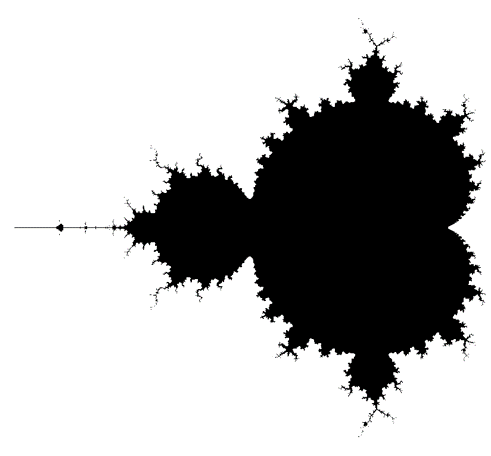
\includegraphics[scale=0.2]{images/ensemble_de_mandelbrot.png}
\end{marginfigure}
Les ensembles de \textsc{Julia} ont les propriétés des fractales, en particulier l'autosimilitude. En revanche, l'ensemble de \textsc{Mandelbrot} est extraordinairement varié: plus l'échelle est grande, plus l'image se complique. On a montré un caractère universel de l'ensemble de \textsc{Mandelbrot}: pour diverses fonctions complexes à un paramètre, on trouve des copies déformées de cet ensemble. 
}

Séries numériques (oraux x-ens)\\
\textsl{
Dans une tentative d'historique des séries numériques, nous pourrions faire remonter leurs origines aux travaux développés dès la fin du \textsc{xvii}$^\e$ siècle autour du comportement asymptotique de sommes du type $\sum\limits_{k=1}^n f(k)$. Quelques années après les travaux de \textsc{Bernoulli} sur ce sujet, \textsc{Euler} et \textsc{Mac-Laurin} produisent indépendamment une \say{ formule sommatoire } obtenue par inversion d'identités tayloriennes:
$$\sum_{k=1}^n f(k) = \int_0^n f + \frac{f(0) + f(n)}{2!} + \frac{f'(n) - f'(0)}{3!} - \frac{f'''(n) - f'''(0)}{6!}\cdots$$
\marginnote[0cm]{
    \note En notant $\mathrm{b}_k$ les nombres de \textsc{Bernoulli},
    $$\sum_{k=0}^{n-1} k^m = \sum_{k=0}^m \binom{m}{k} \mathrm{b}_k \frac{n^{m+1-k}}{m+1-k}.$$
    Pour $|x| < 2 \pi$,
    $$\frac{x}{\e^x-1} = \sum_{k=0}^{+\infty} \mathrm{b}_k \frac{x^k}{k!}.$$
    \note Soit $s \in \Ne$,
    $$\sum_{n=1}^{+\infty} \frac{1}{n^{2s}} = \frac{|\mathrm{b}_{2s}|(2 \pi)^{2s}}{2 (2s)!}.$$
}
Si l'expression générale donnant les coefficients de cette formule leur échappe dans un premier temps, \textsc{Euler} établit leur lien avec les coefficients du développement en série de $\frac{x}{\e^x-1}$ et les nombres de \textsc{Bernoulli}, introduits par celui-ci dans le calcul des sommes $\sum\limits_{k=1}^n k^p$ \note. \textsc{Euler} en déduit, par de jolis calculs, les sommes des séries $\sum\limits_{n=1}^{+\infty} \frac{1}{n^{2s}}$ pour $s$ entier naturel non nul \note.
Cependant, le problème de la convergence des sommes en question n'est jamais au centre de leurs réflexions et l'aspect formel l'emporte, ce qui conduit parfois les plus grands mathématiciens du siècle à commettre de lourdes erreurs. Vers 1768, \textsc{d'Alembert} commence à douter de la validité de l'emploi de séries non convergentes. En 1826, le mot d'\textsc{Abel} illustre parfaitement cette nouvelle préoccupation: \say{ Les séries divergentes sont des inventions du diable, et c'est une honte que l'on ose fonder sur elles la moindre démonstration. On peut en tirer  tout ce qu'on veut quand on les emploie et ce sont elles qui ont produit tant d'échecs et tant de paradoxes } (Œuvres, 1881). \\
Mais ce sont les nécessités du calcul numérique qui imposent vraiment un effort de rigueur dont \textsc{Gauss}, s'étant fait une idée claire de la notion de limite, sera le principal artisan. À partir de là, il paraît naturel d'établir des critères simples de convergence: on en doit plusieurs à \textsc{Cauchy}, et notamment celui qui porte son nom: si la suite de réels positifs $(a_n)_{n \geqslant 0}$ est telle que la limite supérieure de $\sqrt[n]{a_n}$ est strictement inférieure à $1$, alors la série $\sum a_n$ est convergente. \\
(il y a une suite)
}

\newpage

\section{Lemme de \textsc{Cesàro}} \label{lemme_cesaro}
\begin{lemme}
    Soit $(u_n)_{n \in \Ne}$ une suite réelle ou complexe convergeant vers $\ell$.
    Alors la suite de terme général $\frac{1}{n} \sum\limits_{k=1}^{n} u_k$ converge aussi vers $\ell$.
\end{lemme}

\begin{preuve}
    Soit $\varepsilon > 0$. Comme la suite $(u_n)$ converge vers $\ell$, il existe un rang $n_0 \in \Ne$ tel que pour tout $n \geqslant n_0,\ |u_n - \ell| \leqslant \varepsilon$. \\
    Soit $n \geqslant n_0$,
    \begin{align*}
        \left| \frac{1}{n} \sum_{k=1}^n u_k - \ell \right| &= \left| \frac{1}{n} \sum_{k=1}^n (u_k - \ell) \right| \\
        \text{par l'inégalité triangulaire} &\leqslant \frac{1}{n} \sum_{k=1}^n |u_k - \ell| \\
        &\leqslant \frac{1}{n} \Bigg( \underbrace{\sum_{k=1}^{n_0-1} |u_k - \ell|}_{\defeq K} + \sum_{k=n_0}^n \underbrace{|u_k - \ell|}_{\leqslant \varepsilon} \Bigg) \\
        &\leqslant \frac{K}{n} + \varepsilon
    \end{align*}
    Or $\lim\limits_{n \to \infty} \frac{K}{n} = 0$ donc il existe un rang $n_1 \in \Ne$ tel que pour tout $n \geqslant n_1, \left| \frac{K}{n} \right| \leqslant \varepsilon$. \\
    Ainsi pour tout $n \geqslant \max \{ n_0, n_1 \}$, 
    $$\left| \frac{1}{n} \sum_{k=1}^n u_k - \ell \right| \leqslant 2 \varepsilon.$$
    On en déduit que la suite $\Bigg( \frac{1}{n} \sum\limits_{k=1}^{n} u_k \Bigg)_{n \in \Ne}$ converge vers $\ell$.
\end{preuve}

\begin{remarque}
    \textcolor{red}{à réécrire}
    Attention, la réciproque du lemme de \textsc{Cesàro} est fausse. Une suite $(u_n)$ peut converger au sens de \textsc{Cesàro} i.e. $\Bigg( \frac{1}{n} \sum\limits_{k=1}^{n} u_k \Bigg)_{n \in \Ne}$ converge sans pour autant que la suite $(u_n)$ converge. Par exemple, $(u_n) \defeq \left((-1)^n\right)_n$.
\end{remarque}

\section{Série harmonique \& Constante d'\textsc{Euler}}
\begin{defi}{Série harmonique}
    $$\Harmonique_n \defeq \sum_{k=1}^n \frac{1}{k}.$$
\end{defi}

\begin{marginfigure}[6cm]
	\def\a{0.1}
\def\b{11}

\begin{tikzpicture}
    \begin{axis}[width=6.5cm,
        axis lines=middle,
        grid=major,
        xmin=\a, xmax=\b+1,
        ymin=0, ymax=3.5,
        xlabel=$n$, xlabel style={right},
        % ylabel=$y$, ylabel style={above},
        xtick={1,...,11},
        yticklabels={$H_1$, $H_4$, $H_{11}$},
        ytick={1, 1+1/2+1/3+1/4, 1+1/2+1/3+1/4+1/5+1/6+1/7+1/8+1/9+1/10+1/11},
        tick style={thick},
        ticklabel style={font=\normalsize},
    ]
    \addplot[blue,thick,samples=100,domain=\a:\b] {ln(x)} node (m);
    
    \addplot[color=red,mark=*, mark size=1.5pt] coordinates {
    	(1,1)
    	(2,1+1/2)
    	(3,1+1/2+1/3)
    	(4,1+1/2+1/3+1/4)
    	(5,1+1/2+1/3+1/4+1/5)
    	(6,1+1/2+1/3+1/4+1/5+1/6)
    	(7,1+1/2+1/3+1/4+1/5+1/6+1/7)
    	(8,1+1/2+1/3+1/4+1/5+1/6+1/7+1/8)
    	(9,1+1/2+1/3+1/4+1/5+1/6+1/7+1/8+1/9)
    	(10,1+1/2+1/3+1/4+1/5+1/6+1/7+1/8+1/9+1/10)
    	(11,1+1/2+1/3+1/4+1/5+1/6+1/7+1/8+1/9+1/10+1/11)
    } node (l) {};
    \draw [latex-latex] (l) -- (m) node [left] {$\gamma$};
    % \node [left] at (l) {$\ln x$};
    \end{axis}
\end{tikzpicture}
\end{marginfigure}

\begin{prop}{}
    $\lim\limits_{n \to + \infty} \Harmonique_n = + \infty$.
\end{prop}

\begin{prop}{Équivalent de la série harmonique}
    $\forall n \geqslant 1, \ln(n+1) \leqslant \Harmonique_n \leqslant \ln n + 1$ et 
    $$\Harmonique_n \isEquivTo{n \to + \infty} \ln n.$$
\end{prop}

\begin{defi}{Constante d'\textsc{Euler}}
    La constante d'\textsc{Euler} $\gamma$ est définie par:
    $$\gamma \defeq \lim_{n \to \infty} \big(\Harmonique_n - \ln(n) \big) \approx 0,577\ 215\ 664 \dots$$
\end{defi}

\begin{prop}{Développement asymptotique de la série harmonique}
    $\Harmonique_n =_{n \to + \infty} \ln n + \gamma + \frac{1}{2n} + o\left(\frac{1}{n}\right)$.
\end{prop}

\marginnote[2cm]{
    \begin{kaobox}[frametitle=Le théorème de comparaison série / intégrale]
        \cite{acamanes} ch 2. \\
        Soit $f$ une fonction continue par morceaux, décroissante de $\Rp$ à valeurs dans $\Rp$. Alors, la série de terme général 
        $$w_n \defeq \int_{n-1}^n f(t) \d t - f(n)$$
        est convergente. En particulier, $\sum f(n)$ converge si et seulement si $\displaystyle x \mapsto \int_0^x f(t) \d t$ admet une limite finie en $+ \infty$.
    \end{kaobox}
    \begin{methode}
        Le théorème de comparaison série / intégrale permet
        \begin{itemize}
            \item de montrer qu'une série converge ou diverge,
            \item d'obtenir un équivalent d'une somme partielle de série divergente,
            \item d'obtenir un équivalent du reste d'une série convergente.
        \end{itemize}
    \end{methode}
}

\begin{preuve}
    \item Poser $v_n = H_n - \ln(n)$
    \item Montrer que $v_{n+1}-v_n = \mathcal{O}\left(\frac{1}{n^2}\right)$\\
    \begin{align*}
        v_n &= \sum_{k=1}^n\frac{1}{k} -\ln(n) \\
        &= \sum_{k=1}^n \frac{1}{k} -\sum_{k=1}^n  \ln\left( \frac{k+1}{k} \right) \\
        &= \frac{1}{n} + \sum_{k=1}^n \underbrace{\left( \frac{1}{k} - \ln\left(1-\frac{1}{k}\right)\right)}_{\mathcal{O}\left(\frac{1}{k^2}\right)}
    \end{align*}
    On peut aussi montrer...
    \item ... la décroissance de la suite $(v_n)$. \\
    Soit $n \in \N$. 
    $$v_n - v_{n+1} = \ln(n+1) - \ln(n) - \frac{1}{n+1}$$
    Deux méthodes:
    \begin{itemize}
        \item On transforme $\ln(n+1) - \ln(n)$ en intégrale:
        $$v_n - v_{n+1} = \int_{n}^{n+1} \underbrace{\left( \frac{1}{t} - \frac{1}{n+1} \right)}_{\geqslant 0} \d t > 0.$$
        \item D'après le \textbf{théorème des accroissements finis}, il existe $c \in ]n, n+1[$ tel que 
        $$\ln(n+1) - \ln(n) = \ln'(c)((n+1) - n) = \frac{1}{c}$$
        d'où l'on tire que 
        $$v_n - v_{n+1} = \frac{1}{c} - \frac{1}{n+1} > 0.$$
    \end{itemize}
    \item ... que $\forall n \in \Ne,\ \ln(n+1) \leqslant H_n \leqslant \ln(n) + 1$ grâce à l'\textbf{encadrement de l'intégrale} sur $[k, k+1]$ de la fonction $t \mapsto \frac{1}{t}$.
\end{preuve}

\marginnote[-1cm]{\url{https://www.maths-france.fr/MathSpe/GrandsClassiquesDeConcours/SeriesNumeriques/SerieHarmonique.pdf}}

\begin{exercice}
    \marginnote[0cm]{\cite{exos_oraux} p. 334}
    Montrer que l'intégrale $\displaystyle \int_1^{+\infty} \bigg( \frac{1}{\lfloor x \rfloor} - \frac{1}{x}\bigg) \d x$ est égale à $\gamma$.
\end{exercice}

\begin{methode}
    Quand un exercice amène à manipuler des parties entières, il est très souvent judicieux d'utiliser les encadrements suivants
    $$x-1 < \lfloor x \rfloor \leqslant x,$$
    $$\lfloor x \rfloor \leqslant x < \lfloor x \rfloor + 1.$$
\end{methode}

\begin{solution}
\end{solution}

\section{Séries de \textsc{Bertrand}}
\begin{defi}{Séries de \textsc{Bertrand}}
    Soient $\alpha$ et $\beta$ deux réels. On nomme \emph{série de \textsc{Bertrand}} la série de terme général $\displaystyle \frac{1}{n^\alpha \ln^\beta (n)}$ pour $n \geqslant 2$. 
\end{defi}

\begin{theo}{}
    La série de \textsc{Bertrand} converge si et seulement si \begin{cases} \alpha > 1 \\
    \text{ou} \\ \alpha = 1 \text{ et } \beta > 1 \end{cases}.
\end{theo}

\begin{preuve}
    Distinguons trois cas selon les valeurs prises par $\alpha$:
    \begin{enumerate}
        \item[$\rhd$] si $\alpha > 1$, soit $\gamma \in ]1, \alpha[$. Par croissances comparées,
        $$\displaystyle \frac{1}{t^{\alpha} \ln^{\beta} (t)} = o_{+ \infty} \left( \frac{1}{t^{\gamma}} \right).$$
        Or, d'après le théorème de \textsc{Riemann}, la fonction $t \mapsto \frac{1}{t^\gamma}$ est intégrable sur $[2, +\infty[$ car $\gamma > 1$. Ainsi, en appliquant les théorèmes de comparaison, $\int_2^{+ \infty} f$ converge.
        \item[$\rhd$] si $\alpha < 1$, soit $\gamma \in ]\alpha, 1[$.Par croissances comparées,
        $t^{\gamma} f(t) \xrightarrow[t \to + \infty]{} + \infty$
        donc à partir d'un certain rang, $f(t) \geqslant \frac{1}{t^{\gamma}} > 0$. Or, d'après le théorème de \textsc{Riemann}, la fonction $t \mapsto \frac{1}{t^\gamma}$ n'est intégrable pas sur $[2, +\infty[$ car $\gamma < 1$. Ainsi, en appliquant les théorèmes de comparaison (les intégrandes sont positives), $\int_2^{+ \infty} f$ diverge.
        \item[$\rhd$] si $\alpha = 1$, revenons aux intégrales partielles:
        $$\int_{2}^{X} \frac{1}{t \ln^{\beta} (t)} \d t = 
        \begin{cases}
            \left[ \frac{\ln ^{1-\beta} (t)}{1-\beta} \right]_2 ^X & \text{si } \beta \not = 1, \\
            \left[\ln (\ln(t)) \right]_2 ^X & \text{si } \beta = 1.
        \end{cases}
        $$
        On en déduit que l'intégrale de la fonction $t \mapsto \frac{1}{t \ln^{\beta} (t)}$ converge sur $[2, + \infty[$ si et seulement si $\beta > 1$.
    \end{enumerate}
\end{preuve}


\begin{exercice}
    \marginnote[0cm]{\cite{acamanes}}
    On note $h : x \mapsto \sum\limits_{n=2}^{+ \infty} \frac{1}{n^x \ln n}$.
    \begin{enumerate}
        \item Étudier la continuité de $h$ sur son domaine de définition.
        \item Étudier les limites de $h$ aux bornes de son intervalle de définition.
        \item Déterminer des équivalents de $h$ aux bornes de son intervalle de définition.
    \end{enumerate}
\end{exercice}

\begin{solution}
\begin{enumerate}
    On note $f_x : t \mapsto \frac{1}{t^x \ln t}$.
    \item D'après le théorème de \textsc{Bertrand} sur les séries numériques, l'ensemble de définition de $h$ est $\mathcal{D}_h \defeq ]1, + \infty[$. \\
    Soit $a > 1$. On se place sur $I \defeq [a, +\infty[$. Pour tout $x \in I$,
    $$\left| \frac{1}{n^x \ln n} \right| \leqslant \frac{1}{n^\alpha \ln n}$$
    comme $a > 1$, d'après le théorème de \textsc{Bertrand} sur les séries numériques, la série du terme majorant converge et donc par théorème de comparaison, la suite $(f_x)$ converge normalement sur tout segment de la forme de $I$. On en déduit que $h$ est continue sur $\mathcal{D}_h$. 
    \begin{itemize}
        \item En $+ \infty$: comme la série des $f_x$ converge uniformément sur $[2, + \infty[$ (on aurait pu choisir une valeur que $2$), d'après le théorème de la double limite
        $$\lim_{x \to + \infty} h(x) = \sum_{n=2}^{+ \infty} \left[\lim_{x \to +\infty} f_x(n) \right] = 0.$$
        \item En $1^+$: On montre que la fonction $f_x$ est décroissante et donc $h$ aussi. On note $\ell \defeq \lim\limits_{1^+} h$. D'après le théorème de la limite monotone, $\ell \in \R \cup \{ + \infty \}$. \\
        Supponson que $\ell \in \R$, alors
        $$h(x) = \sum_{n=2}^{+\infty} \frac{1}{n^x \ln n} \geqslant \sum_{n=2}^N \frac{1}{n^x \ln n}$$
        et en passant à la limite quand $x$ tend vers $1^+$ dans l'inégalité (ce qui est licite) on obtient
        $$\ell \geqslant \sum_{n=2}^N \frac{1}{n \ln n}.$$
        Nous aboutissons donc à une contradiction car la somme minorante diverge quand $N$ tend vers $+ \infty$. Finalement,
        $$\lim_{1^+} h = + \infty.$$
    \end{itemize}
    \item 
    \begin{itemize}
        \item En $+ \infty$: on intuite que la premier terme de la somme domine les autres. On a
        $$2^x \ln(2) h(x) = 1 + \sum_{n=3}^{+\infty} \left(\frac{2}{n}\right)^x \frac{\ln 2}{\ln n}.$$
        On peut montrer(...) que la somme converge normalement sur $[2, +\infty[$. On en déduit que 
        $$h(x) \isEquivTo{+\infty} \frac{1}{2^x \ln 2}.$$
        \item En $1^+$: un encadrement par la méthode des rectangles permet de trouver
        $$\int_{3}^{+\infty} f_x(t) \d t + \frac{1}{2^x \ln 2} \leqslant h(x) \leqslant \int_{2}^{+\infty} f_x(t) \d t + \frac{1}{2^x \ln 2}.$$
        On en déduit que 
        $$h(x) \isEquivTo{1^+} \int_2^{+\infty} f_x(t) \d t$$
        soit après calculs (...)
        $$h(x) \isEquivTo{1^+} - \ln(x-1).$$
    \end{itemize}
\end{enumerate}
\end{solution}

\section{Deux sommes} \label{deux_sommes}
\begin{exercice}
    Calculer $\displaystyle \sum_{n=1}^{+\infty} \frac{(-1)^n}{n}$ et $\displaystyle \sum_{n=0}^{+\infty} \frac{(-1)^n}{2n+1}$.
\end{exercice}

\begin{elem_sol}
    \begin{itemize}
        \item Exprimer les termes généraux avec une intégrale. 
        \item (1)$= -\ln(2)$, (2)$= \frac{\pi}{4}$.
    \end{itemize}
\end{elem_sol}


\section{Sommation des relations de comparaison} \label{sommation_relations_comparaison}
\begin{tcolorbox}
    Soient $(a_n)_{n \in \Ne}$ et $(b_n)_{n \in \Ne}$ deux suites à valeurs positives telles que $a_n \sim b_n$.\\
    Si $ \sum a_k$ diverge, alors $\sum\limits_{k=1}^{n} a_k \sim \sum\limits_{k=1}^{n} b_k$. \\
    Si $ \sum a_k$ converge, alors $\sum\limits_{k=n+1}^{+ \infty} a_k \sim \sum\limits_{k=n+1}^{+ \infty} b_k$. \\
    \emph{Il y a des résultats analogues si $u_n = o(v_n)$ ou si $u_n = \mathcal{O}(v_n)$.}
\end{tcolorbox}

\begin{itemize}
    \item Revenir à la définition de l'équivalence avec le $o$: $a_n \sim b_n \Longleftrightarrow a_n -b_n = o(b_n)$.
\end{itemize}

\section{Règle de \textsc{Raabe-Duhamel}}
\begin{theo}
    Soit $\alpha$ un réel et $(u_n)_{n \in \N}$ une suite de réels strictement positifs. On suppose que
    $$\displaystyle \frac{u_{n+1}}{u_n} = 1 - \frac{\alpha}{n} + \mathcal{O} \left( \frac{1}{n^2} \right).$$ Alors $\sum u_n$ converge si et seulement si $\alpha > 1$. 
\end{theo}
\marginnote[-1cm]{Voir exercice 3.43. \cite{oraux_x_ens_3}}
\begin{enumerate}
    \item[($\Rightarrow$)] Montrer que si $u_n=\frac{K}{n^{\alpha}}$ avec $K>0$ et $\alpha > 1$ alors $(u_n)$ vérifie la relation.
    \item[($\Leftarrow$)] Soit $(v_n)$ une suite vérifiant les hypothèses. Montrer qu'il existe $K>0$ tel que $v_n \sim \frac{K}{n^{\alpha}}$ avec $\alpha > 0$. Pour cela, étudier la série de terme général $\ln (v_n)$.
\end{enumerate}

Être capable de donner deux séries montrant qu'on ne peut pas conclure si $\alpha=1$.

\section{Suites sous-additive}
\emph{Exercice 2. TD I \cite{acamanes}}\\

\begin{defi}
    Une suite $(u_n)_{n\geqslant1}$ est dite \emph{sous-additive} si pour tout couple d'entiers non nuls $(n, m)$, $u_{n+m} \leqslant u_n + u_m$.
\end{defi}

\begin{exercice}
    Soit $(u_n)_{n \geqslant 1}$ une suite sous-additive. On pose $b_n = \min\limits_{k \in \llbracket 1, n \rrbracket} \frac{u_k}{k}$.
    \begin{enumerate}
        \item \begin{enumerate}
            \item Soit $\alpha \in \Rp$ et, pour $n \in \Ne, t_n = n^{\alpha}$. Montrer que $(t_n)$ est sous-additive si et seulement si $\alpha \leqslant 1$. Déterminer alors la limite de la suite $(t_n/n)$.
            \item Soit $(w_n)$ une suite réelle telle que pour tout $(n,m) \in (\Ne)^2, w_{n+m} = w_n + w_m$. Montrer que $(w_n)$ est sous-additive et calculer la limite de la suite $(w_n / n)$.
        \end{enumerate}
        \item Montrer qu'il existe $\ell \in \R \cup \{ - \infty \}$ telle que $\lim\limits_{n \to +\infty} v_n = \ell$.
        \item Montrer que pour tout $(m,n) \in (\Ne)^2, u_{nm} \leqslant m u_n$.
        \item On suppose que $\ell \not= - \infty$. Soit $\varepsilon > 0$.
        \begin{enumerate}
            \item Montrer qu'il existe $m \in \N$ tel que $\frac{u_m}{m} \leqslant \ell + \varepsilon$. 
            \item En utilisant le théorème de la division euclidienne, montrer que $\left( \frac{u_n}{n} \right)_{n \geqslant 1}$ converge vers $\ell$.
        \end{enumerate}
    \end{enumerate}
\end{exercice}

\begin{solution}
    1.a)\\ 
    \indent $(\Leftarrow)$ Étudier les cas où $n=m$.\\
    \indent $(\Rightarrow)$ Étudier la fonction $f:x \mapsto 1+x^{\alpha} - (1+x)^{\alpha}$.\\
    1.b)\\
    \indent Étudier le cas où $m=1$ et montrer que $w_n = n w_1$.\\
    2)\\
    \indent Montrer que la suite $(v_n)$ est décroissante.\\ 
    4.b)\\
    \indent Soit $(n, m) \in (\Ne)^2$. D'après le théorème de la division euclidienne, il existe un unique couple $(k, r) \in \Ne \times \llbracket0, m-1 \rrbracket$ tel que $n=km+r$.\\
    \indent Utiliser successivment la définition d'une suite sous-additive et les résultats des questions 3) et 4.a).
\end{solution}


\section{Étude de la suite de terme général \texorpdfstring{$\left( \frac{1}{b-a} \int_{a}^{b} f(x)^n \d x \right)^{1/n}$}{égal à une intégrale}}
\emph{Exercice 9. TD I}\\
La fonction $f$ est supposée continue et positive sur $[a, b]$.

\begin{itemize}
    \item La démarche générale consiste à encadrer $u_n$. 
    \item \underline{Majoration:} $f$ est continue sur un segment donc est en particuler bornée par un réel positif $M$. On peut montrer que $u_n \leqslant M$ \emph{(ne pas oublier l'argument de la continuité lors du passage à l'intégrale)}.
    \item \underline{Minoration:} soit $\varepsilon > 0$, soit $x_0$ tel que $f(x_0) = M$. Comme $f$ est continue en $x_0$, il existe $[c, d] \subset [a, b]$ tel que $x_0 \in [c, d]$ et pour tout $x \in [c, d]$, $f(x) \geqslant M - \varepsilon$ \emph{(un dessin permet de bien comprendre la stratégie)}.\\
    On peut ensuite montrer que $u_n \geqslant \left(\frac{d-c}{b-a} \right)^{1/n}(M-\varepsilon) \xrightarrow[n \to + \infty]{} M-\varepsilon$.
    \item Finalement, $\boxed{u_n \displaystyle \longrightarrow M = \max_{[ a, b ]} f = \Ninf{f}}$.
\end{itemize}

\section{Transformation d'\textsc{Abel}} \label{transformation_abel}
\marginnote[0cm]{Texte de \cite{oraux_x_ens_3} p. 262.}
La technique des transformations d'\textsc{Abel} peut être vue comme des intégrations par parties discrètes. On s'intéresse à la nature de la série $\sum a_n b_n$ où $(a_n)_{n \in \N}$ et $(b_n)_{n \in \N}$ sont deux suites réelles ou complexes. Pour $n \geqslant 0$ on note $A_n \defeq \sum\limits_{k=0}^n a_k$ la $n$-ième somme partielle de la série $\sum a_n$. On peut alors écrire $a_n = A_n - A_{n-1}$ (avec la convention $A_{-1} = 0$) et ainsi, pour tout entier $N$ on a
\begin{align*}
    \sum_{n=0}^N a_n b_n &= \sum_{n=0}^N (A_n - A_{n-1})b_n =  \sum_{n=0}^N A_n b_n -  \sum_{n=0}^N A_{n-1}b_n \\
    &= \sum_{n=0}^N A_n b_n - \sum_{n=0}^{N-1} A_n b_{n+1} \\
    \sum_{n=0}^N a_n b_n &= A_N b_{N+1} - \sum_{n=0}^N A_n(b_{n+1}-b_n). \quad (\star)
\end{align*}
La suite $(A_n)$ joue le rôle de la \say{ primitive } de $a_n$ et $b_{n+1} - b_n$ celui de la \say{ dérivée } de $b_n$. \\
Une application classique correspond à ce qu'on appelle parfois théorème d'\textsc{Abel} ou test de \textsc{Dirichlet}: 
\begin{theo}
    Lorsque la suite $(b_n)_{n \in \N}$ est décroissante de limite nulle et la suite des sommes partielles $(A_n)$ est bornée, alors la série $\sum a_n b_n$ converge. 
\end{theo}

En effet, dans $(\star)$ le terme $A_N b_{N+1}$ converge vers $0$ quand $N$ tend vers l'infini et la série $\sum A_n(b_n - b_{n+1})$ est absolument convergente car le terme général est un $\mathcal{O}(b_n - b_{n+1})$ avec la série à termes positifs $\sum(b_n - b_{n+1})$ qui est convergente. \\
Appliquons ce théorème aux séries trigonométriques de la forme $\sum \frac{\me^{\mi n x}}{n^\alpha}$ avec $\alpha > 0$ et $x \not \equiv 0 [2\pi]$ en prenant $a_n \defeq \me^{\mi n x}$ et $b_n \defeq \frac{1}{n^\alpha}$. Les sommes partielles $(A_n)$ sont effectivement bornées puisque
$$|A_n| = \left| \sum_{k=0}^n \me^{\mi k x}\right| = \left| \frac{1 - \me^{\mi (n+1)x}}{1-\me^{\mi x}} \right| = \left| \frac{\sin \left( \frac{n+1}{2} x\right)}{\sin \left( \frac{x}{2} \right)} \right| \leqslant \frac{1}{\left| \sin \left( \frac{x}{2} \right) \right|}.$$
Historiquement cette transformation fut utilisée par \textsc{Abel} en 1826 pour donner un exemple de série de fonctions continues dont la somme n'est pas continue \footnote{\textsc{Cauchy} affirme, en 1821, que la somme d'une série de fonctions continue est toujours continue (\textcolor{green}{rajouter la référence})}, à savoir $\sum \frac{\sin nx}{n}$.


\section{Convergence et calcul de  \texorpdfstring{$\sum \frac{r}{2^r}$}{de la série de terme général r/2^r}}
\begin{exercice}
    Montrer la convergence de la série de terme général $\frac{r}{2^r}$ et prouver que $\sum\limits_{r=1}^{+ \infty} \frac{r}{2^r} = 2$. 
\end{exercice}

\marginnote[2cm]{
    \begin{theo}{}
        Soient $\sum u_n$ et $\sum v_n$ deux séries telles que $\sum u_n$ et $\sum v_n$ convergent absolument. Alors, en posant $w_n \defeq \sum\limits_{k=0}^n u_k v_{n-k}$, la série $\sum w_n$ converge absolument et
        $$\sum_{n=0}^{+\infty} u_n \cdot \sum_{n=0}^{+\infty} v_n = \sum_{n=0}^{+\infty} w_n.$$
    \end{theo}
}

\begin{elem_sol}
    Deux méthodes de résolution sont possibles bien que la première soit plus élégante. 
    \begin{itemize}
        \item La série $\sum \frac{1}{2^r}$ est une série géométrique absolument convergente. Ainsi, d'après le résultat sur les produits de \textsc{Cauchy}, 
        $$\sum_{r=0}^{+ \infty} \frac{r}{2^{r-1}} = \sum_{r=0}^{+ \infty} \sum_{k=0}^{r} \frac{1}{2^k \cdot 2^{r-k}} = \left( \sum_{r=0}^{+ \infty} \frac{1}{2^r} \right)^2 = 4.$$
        \item On peut également étudier la fonction $g : x \to \sum\limits_{r=0}^{n} \frac{x^r}{2^r}$.
    \end{itemize}
\end{elem_sol}


\section{Suites du type \texorpdfstring{$f(x_n) = n$}{f(x_n) = n}}
\begin{itemize}
    \item \emph{Exercice X 1 p.226 de \cite{exos_oraux}}\\
    Soit $n \in \N$, montrer que l'équation $x \me^x = n$ admet une unique solution $x_n \in \R$, en donner un équivalent puis un équivalent de $y_n = x_n - \ln(n)$. 
    \item Soit $n \in \Ne$, montrer que l'équation $x + \ln(x) = n$ admet une unique solution $x_n \in \R$, en donner un équivalent.
\end{itemize}

\section{Suites définies implicitement}

\begin{methode}
    \marginnote[0cm]{Texte de \cite{oraux_x_ens_3} p. 181.}
    \begin{enumerate}
        \item Montrer l'existence de $x_n$
        \item Démontrer la convergence de la suite $x_n$
        \item Déterminer un équivalent 
        \item Déterminer un développement asymptotique de $x_n$ \\
        Pour cela il faut commencer par déterminer dans la relation qui définit $x_n$ quels sont les termes prépondérants. 
    \end{enumerate}
\end{methode}

\section{Sommation par paquets}
\begin{exercice}
    \marginnote[0cm]{\cite{exos_oraux} p. 340}
    Soit $\sum\limits_{n \geqslant 1} u_n$ une série à termes réels positifs, telle que $(u_n)_{n \geqslant 1}$ est décroissante. Montrer que les séries $\sum\limits_{n \geqslant 1} u_n$ et $\sum\limits_{n \geqslant 2} 2^n u_{2^n}$ sont de même nature. 
\end{exercice}

\section{Plan d'étude des suites \texorpdfstring{$u_{n+1} = f(u_n)$}{u_(n+1) = f(u_n)}}

La fonction $f$ doit être continue. 
\begin{enumerate}
    \item Trouver un invervalle $I$ stable par $f$ ($f(I) \subset I$). Le segment $I$ doit contenir, au moins à partir d'un certain rang, tous les termes de la suite.
    \item Recherche des points fixes de la fonction $f$ dans $I$.
    \item ...
\end{enumerate}

\section{Techniques classiques}
\marginnote[0cm]{Arnaud Guyader}
\subsection{Développements asymptotiques}

Dans de nombreuses situations, on conclut sur la nature d'une série en se ramenant à une série plus simple. On a vu que pour les séries à termers positifs, il suffit de se ramener à un équivalent. Ceci n'est plus le cas avec des séries à termes de signe quelconque. Par ailleurs, un équivalent correspond à une approximation au premier ordre, laquelle ne permet pas forcément de conclure. \\
Dans ces deux situations, il suffit souvent d'écrire un développement asymptotique du terme général, c'est-à-dire d'être plus précis dans l'approximation. Celui-ci est généralement en $\frac{1}{n}$ ou en $\frac{1}{\sqrt{n}}$ et s'arrête au premier terme absolument convergent, en $\frac{1}{n^2}$ ou $\frac{1}{n^{3/2}}$.

Exemples: \\
$$\sum_{n \geqslant 2} \ln \left(1 + \frac{(-1)^n}{\sqrt{n}}\right) \text{ est divergente}.$$
$$\sum_{n \geqslant 1} \left(\frac{1}{\sqrt{n}} - \sqrt{n} \sin \frac{1}{n} \right) \text{ est absolument convergente}.$$

\subsection{Groupements de termes}

Considérons une série numérique $\sum u_n$ dont on veut déterminer la nature. On commence par s'assurer que le terme général $(u_n)$ tend vers zéro, sinon la série est trivialement divergente. Ceci fait, il faudrait montrer que la suite $(s_N)$ des sommes partielles est convergente, ce qui n'est pas toujours facile. En particulier, il est parfois plus simple de montrer qu'une sous-suite de $(s_N)$ converge, par exemple en effectuant des regroupements de termes, et de conclure ensuite. \\
Cadre typique d'application: on réussit à montrer que $(s_{2N})$ converge, disons vers $s$. Alors pour la sous-suite $(s_{2N+1})$, il suffit d'écrire:
$$s_{2N+1} = s_{2N} + u_{2N+1},$$
et si la série ne diverge par trivialement, on a
$$\lim_{N \to + \infty} s_{2N+1} = \lim_{N \to + \infty} s_{2N} = s,$$
c'est-à-dire que 
$$\lim_{N \to \infty} s_N = s,$$
la série converge. 

\section{Complément: Suites de \textsc{Cauchy}}

Issu du cours de Sophie \textsc{Dede} (Stanislas Paris). \\
\begin{defi}{Suite de \textsc{Cauchy}}
    Soit $(u_n)_{n \in \N}$ une suite réelle. La suite $(u_n)_{n \in \N}$ est dite de \textsc{Cauchy} si et seulement si :
    $$\forall \varepsilon > 0, \exists N \in \N, \forall n \geqslant N, \forall p \in \N, |u_{n+p} - u_n| \leqslant \varepsilon.$$
\end{defi}

\begin{prop}{}
    Soit $(u_n)_{n \in \N}$ une suite réelle convergente. Alors  $(u_n)_{n \in \N}$ est une suite de \textsc{Cauchy}.
\end{prop}

\begin{preuve}
    Soit $\ell \defeq \lim\limits_{n \to \infty} u_n:\ \forall \varepsilon > 0, \exists N \in \N, \forall n \geqslant N, |u_n - \ell| \leqslant \frac{\varepsilon}{2}$. \\
    Donc, à l'aide de l'inégalité triangulaire, on obtient,
    $$\forall n \geqslant N, \forall p \in \N, |u_{n+p} - u_n| \leqslant |u_{n+p} - \ell| + |u_n - \ell| \leqslant \varepsilon,$$
    car $n + p \geqslant N$.
\end{preuve}

\begin{theo}{}
    Toute suite réelle de \textsc{Cauchy} converge dans $\R$.
\end{theo}

Pour prouver ce résultat, on commence par démontrer deux lemmes.

\begin{lemme}
    Soit $(u_n)_{n \in \N}$ une suite réelle de \textsc{Cauchy} qui admet une sous-suite convergente dans $\R$, alors $(u_n)_{n \in \N}$ est convergente. 
\end{lemme}

\begin{preuve}
    Soit $\varphi : \N \to \N$ strictement croissante telle que $\left( u_{\varphi(n)} \right)_{n \in \N}$ converge vers $\ell \in \R$:
    $$\forall \varepsilon > 0, \exists N \in \N, n \geqslant N \Rightarrow |u_{\varphi(n)} - \ell| \leqslant \varepsilon.$$
    La suite $(u_n)_{n \in \N}$ est de \textsc{Cauchy}, donc: $\forall \varepsilon > 0, \exists N' \in \N, \forall n \geqslant N', \forall p \in \N, |u_{n+p} - u_n| \leqslant \varepsilon$. \\
    De plus, $\forall n \in \N, \varphi(n) \geqslant n$, donc si $n \geqslant \max \{ N, N' \}$, on a:
    $$\forall p \in \N, |u_{\varphi(n) + p} - \ell| \leqslant |u_{\varphi(n) + p} - u_{\varphi(n)}| + |u_{\varphi(n)} - \ell| \leqslant 2 \varepsilon.$$
    Donc, en notant $N'' \defeq \varphi \big( \max \{ N, N' \} \big)$, on a:
    $$\forall p \in \N, |u_{N'' + p} - \ell| \leqslant 2 \varepsilon.$$
    Ainsi, 
    $$\forall n \geqslant N'', |u_n - \ell| \leqslant 2 \varepsilon,$$
    donc, $(u_n)_{n \in \N}$ converge vers $\ell$.
\end{preuve}

\begin{lemme}
    Toute suite de \textsc{Cauchy} est bornée.
\end{lemme}

\begin{preuve}
    Soit $(u_n)_{n \in \N}$ une suite réelle de \textsc{Cauchy}:
    $$\forall \varepsilon > 0, \exists N \in \N, \forall n \geqslant N, \forall p \in \N, |u_{n+p} - u_n| \leqslant \varepsilon.$$
    Donc, 
    $$\exists N \in \N, \forall p \in \N, |u_{N+p} - u_N| \leqslant 1.$$
    Ainsi, 
    $$\forall p \in \N, |u_{N+p}| \leqslant 1 + |u_N|.$$
    On en déduit:
    $$\forall n \in \N, |u_n| \leqslant \max \big\{ |u_0|, \dots, |u{N-1}|, |u_N|+1 \big\}.$$
\end{preuve}

Revenons à la démonstration du théorème.

\begin{preuve}
    Soit $(u_n)_{n \in \N}$ une suite réelle de \textsc{Cauchy}. D'après le second lemme, la suite $(u_n)_{n \in \N}$ est bornée donc d'après le théorème de \textsc{Bolzano}-\textsc{Weierstrass}, $(u_n)_{n \in \N}$ admet une sous-suite convergente. Donc, d'après le premier lemme, $(u_n)_{n \in \N}$ est convergente. 
\end{preuve}

\begin{defi}{Ensemble complet}
    On dit alors que $\R$ est complet, c'est-à-dire que toute suite de \textsc{Cauchy} réelle est convergente et admet une limite dans $\R$. 
\end{defi}

\begin{remarque}
    $$\forall \varepsilon > 0, \exists N \in \N, n \geqslant N \Rightarrow |u_{n+1} - u_n| \leqslant \varepsilon$$
    n'entraîne pas la convergence de la suite $(u_n)_{n \in \N}$.
\end{remarque}

En effet, si pour tout $n \in \N$ on pose $u_n \defeq \ln(n+1)$ alors
$$\forall n \in \N, |u_{n+1} - u_n| \leqslant \ln \left( 1 + \frac{1}{n+1} \right) \leqslant \frac{1}{n+1}.$$
On en déduit
$$\forall \varepsilon > 0, n \geqslant \left \lfloor \frac{1}{\varepsilon} \right \rfloor \Rightarrow |u_{n+1} - u_n| \leqslant \varepsilon,$$
et pourtant la suite $(u_n)_{n \in \N}$ diverge vers $+ \infty$.

\begin{remarque}
    $\Q$ n'est pas complet.
\end{remarque}

En effet, si pour tout $n \in \N$, on pose $u_n \defeq \frac{\lfloor 10^n \sqrt{2} \rfloor}{10^n}$. La suite $(u_n)_{n \in \N}$ est à valeurs rationnelles et converge vers $\sqrt{2} \in \R \setminus \Q$. 